\documentclass[twoside]{book}

% Packages required by doxygen
\usepackage{calc}
\usepackage{doxygen}
\usepackage{graphicx}
\usepackage[utf8]{inputenc}
\usepackage{makeidx}
\usepackage{multicol}
\usepackage{multirow}
\usepackage{textcomp}
\usepackage[table]{xcolor}

% Font selection
\usepackage[T1]{fontenc}
\usepackage{mathptmx}
\usepackage[scaled=.90]{helvet}
\usepackage{courier}
\usepackage{amssymb}
\usepackage{sectsty}
\renewcommand{\familydefault}{\sfdefault}
\allsectionsfont{%
  \fontseries{bc}\selectfont%
  \color{darkgray}%
}
\renewcommand{\DoxyLabelFont}{%
  \fontseries{bc}\selectfont%
  \color{darkgray}%
}

% Page & text layout
\usepackage{geometry}
\geometry{%
  a4paper,%
  top=2.5cm,%
  bottom=2.5cm,%
  left=2.5cm,%
  right=2.5cm%
}
\tolerance=750
\hfuzz=15pt
\hbadness=750
\setlength{\emergencystretch}{15pt}
\setlength{\parindent}{0cm}
\setlength{\parskip}{0.2cm}
\makeatletter
\renewcommand{\paragraph}{%
  \@startsection{paragraph}{4}{0ex}{-1.0ex}{1.0ex}{%
    \normalfont\normalsize\bfseries\SS@parafont%
  }%
}
\renewcommand{\subparagraph}{%
  \@startsection{subparagraph}{5}{0ex}{-1.0ex}{1.0ex}{%
    \normalfont\normalsize\bfseries\SS@subparafont%
  }%
}
\makeatother

% Headers & footers
\usepackage{fancyhdr}
\pagestyle{fancyplain}
\fancyhead[LE]{\fancyplain{}{\bfseries\thepage}}
\fancyhead[CE]{\fancyplain{}{}}
\fancyhead[RE]{\fancyplain{}{\bfseries\leftmark}}
\fancyhead[LO]{\fancyplain{}{\bfseries\rightmark}}
\fancyhead[CO]{\fancyplain{}{}}
\fancyhead[RO]{\fancyplain{}{\bfseries\thepage}}
\fancyfoot[LE]{\fancyplain{}{}}
\fancyfoot[CE]{\fancyplain{}{}}
\fancyfoot[RE]{\fancyplain{}{\bfseries\scriptsize Generated on Tue Apr 21 2015 00\-:16\-:40 for My Project by Doxygen }}
\fancyfoot[LO]{\fancyplain{}{\bfseries\scriptsize Generated on Tue Apr 21 2015 00\-:16\-:40 for My Project by Doxygen }}
\fancyfoot[CO]{\fancyplain{}{}}
\fancyfoot[RO]{\fancyplain{}{}}
\renewcommand{\footrulewidth}{0.4pt}
\renewcommand{\chaptermark}[1]{%
  \markboth{#1}{}%
}
\renewcommand{\sectionmark}[1]{%
  \markright{\thesection\ #1}%
}

% Indices & bibliography
\usepackage{natbib}
\usepackage[titles]{tocloft}
\setcounter{tocdepth}{3}
\setcounter{secnumdepth}{5}
\makeindex

% Hyperlinks (required, but should be loaded last)
\usepackage{ifpdf}
\ifpdf
  \usepackage[pdftex,pagebackref=true]{hyperref}
\else
  \usepackage[ps2pdf,pagebackref=true]{hyperref}
\fi
\hypersetup{%
  colorlinks=true,%
  linkcolor=blue,%
  citecolor=blue,%
  unicode%
}

% Custom commands
\newcommand{\clearemptydoublepage}{%
  \newpage{\pagestyle{empty}\cleardoublepage}%
}


%===== C O N T E N T S =====

\begin{document}

% Titlepage & ToC
\hypersetup{pageanchor=false}
\pagenumbering{roman}
\begin{titlepage}
\vspace*{7cm}
\begin{center}%
{\Large My Project }\\
\vspace*{1cm}
{\large Generated by Doxygen 1.8.6}\\
\vspace*{0.5cm}
{\small Tue Apr 21 2015 00:16:40}\\
\end{center}
\end{titlepage}
\clearemptydoublepage
\tableofcontents
\clearemptydoublepage
\pagenumbering{arabic}
\hypersetup{pageanchor=true}

%--- Begin generated contents ---
\chapter{Parser Project Documentation}
\label{index}\hypertarget{index}{}This repository contains the basic steps in of \hyperlink{namespaceNLP}{N\-L\-P}. Tokenizer and Tagger 
\chapter{R\-E\-A\-D\-M\-E}
\label{md_README}
\hypertarget{md_README}{}
Join our online chat at \href{https://gitter.im/nlp}{\tt !\mbox{[}Gitter\mbox{]}(https\-://badges.\-gitter.\-im/\-N\-L\-P/gitter.\-svg)}

\section*{Parser}

\hyperlink{namespaceNLP}{N\-L\-P} Parser (syntactic analysis)

\section*{Check Wiki for documentation}
\chapter{Namespace Index}
\section{Namespace List}
Here is a list of all documented namespaces with brief descriptions\-:\begin{DoxyCompactList}
\item\contentsline{section}{\hyperlink{namespaceNLP}{N\-L\-P} }{\pageref{namespaceNLP}}{}
\end{DoxyCompactList}

\chapter{Hierarchical Index}
\section{Class Hierarchy}
This inheritance list is sorted roughly, but not completely, alphabetically\-:\begin{DoxyCompactList}
\item \contentsline{section}{N\-L\-P\-:\-:Converter}{\pageref{classNLP_1_1Converter}}{}
\item \contentsline{section}{F\-Tokenize}{\pageref{classFTokenize}}{}
\item \contentsline{section}{S\-Tokenize}{\pageref{classSTokenize}}{}
\item \contentsline{section}{Token}{\pageref{classToken}}{}
\begin{DoxyCompactList}
\item \contentsline{section}{N\-L\-P\-:\-:Word}{\pageref{classNLP_1_1Word}}{}
\end{DoxyCompactList}
\end{DoxyCompactList}

\chapter{Class Index}
\section{Class List}
Here are the classes, structs, unions and interfaces with brief descriptions\-:\begin{DoxyCompactList}
\item\contentsline{section}{\hyperlink{classNLP_1_1Converter}{N\-L\-P\-::\-Converter} \\*Class to process a sentence and generate the list of words and it's corresponding datas }{\pageref{classNLP_1_1Converter}}{}
\item\contentsline{section}{\hyperlink{classFTokenize}{F\-Tokenize} }{\pageref{classFTokenize}}{}
\item\contentsline{section}{\hyperlink{classSTokenize}{S\-Tokenize} }{\pageref{classSTokenize}}{}
\item\contentsline{section}{\hyperlink{classToken}{Token} }{\pageref{classToken}}{}
\item\contentsline{section}{\hyperlink{classNLP_1_1Word}{N\-L\-P\-::\-Word} \\*A Class to store token and its corresponding tags and definitions }{\pageref{classNLP_1_1Word}}{}
\end{DoxyCompactList}

\chapter{Namespace Documentation}
\hypertarget{namespaceNLP}{\section{N\-L\-P Namespace Reference}
\label{namespaceNLP}\index{N\-L\-P@{N\-L\-P}}
}
\subsection*{Classes}
\begin{DoxyCompactItemize}
\item 
class \hyperlink{classNLP_1_1Converter}{Converter}
\begin{DoxyCompactList}\small\item\em Class to process a sentence and generate the list of words and it's corresponding datas. \end{DoxyCompactList}\item 
class \hyperlink{classNLP_1_1Word}{Word}
\begin{DoxyCompactList}\small\item\em A Class to store token and its corresponding tags and definitions. \end{DoxyCompactList}\end{DoxyCompactItemize}
\subsection*{Enumerations}
\begin{DoxyCompactItemize}
\item 
enum {\bfseries Word\-Type} \{ \\*
{\bfseries others} = 0, 
{\bfseries adjective}, 
{\bfseries adverb}, 
{\bfseries conjunction}, 
\\*
{\bfseries dative}, 
{\bfseries noun}, 
{\bfseries interjections}, 
{\bfseries imperative}, 
\\*
{\bfseries particple}, 
{\bfseries preposition}, 
{\bfseries pronoun}, 
{\bfseries plural}, 
\\*
{\bfseries singular}, 
{\bfseries verb}, 
{\bfseries transitive}, 
{\bfseries intransitive}, 
\\*
{\bfseries interrogative}, 
{\bfseries object}, 
{\bfseries I\-G\-N\-O\-R\-E\-T\-H\-I\-S}
 \}
\end{DoxyCompactItemize}
\subsection*{Variables}
\begin{DoxyCompactItemize}
\item 
\hypertarget{namespaceNLP_a2a777e12096928b1e7d904b6d6484556}{const Q\-String {\bfseries D\-B\-\_\-\-P\-A\-T\-H} = \char`\"{}../../en\-\_\-db.\-sqlite\char`\"{}}\label{namespaceNLP_a2a777e12096928b1e7d904b6d6484556}

\end{DoxyCompactItemize}


\subsection{Detailed Description}
word.\-cpp Copyright (C) 2015 Tony Lim \href{mailto:atomictheorist@gmail.com}{\tt atomictheorist@gmail.\-com}

Distributed under terms of the M\-I\-T license. 
\chapter{Class Documentation}
\hypertarget{classNLP_1_1Converter}{\section{N\-L\-P\-:\-:Converter Class Reference}
\label{classNLP_1_1Converter}\index{N\-L\-P\-::\-Converter@{N\-L\-P\-::\-Converter}}
}


Class to process a sentence and generate the list of words and it's corresponding datas.  




{\ttfamily \#include $<$converter.\-h$>$}

\subsection*{Public Member Functions}
\begin{DoxyCompactItemize}
\item 
\hyperlink{classNLP_1_1Converter_a7da0cffead471133931098b132ed9631}{Converter} (const string \&sentence)
\begin{DoxyCompactList}\small\item\em Constructor first setup the list of tokens from a sentence Then, connect Dictionary database to a private Q\-Sql\-Database variable This database will be used by any query created in this class. \end{DoxyCompactList}\item 
list$<$ \hyperlink{classNLP_1_1Word}{Word} $>$ \hyperlink{classNLP_1_1Converter_a136cb6f6f522af85ec0a4cc4dac61645}{get\-Words} ()
\begin{DoxyCompactList}\small\item\em Function to finalize the list of words to be returned, along with its corresponding roles. \end{DoxyCompactList}\item 
\hypertarget{classNLP_1_1Converter_a417bff3c0e0b23e25e231fa088c0cd05}{\hyperlink{classNLP_1_1Converter_a417bff3c0e0b23e25e231fa088c0cd05}{$\sim$\-Converter} ()}\label{classNLP_1_1Converter_a417bff3c0e0b23e25e231fa088c0cd05}

\begin{DoxyCompactList}\small\item\em no dynamic thing to destroy for now \end{DoxyCompactList}\end{DoxyCompactItemize}


\subsection{Detailed Description}
Class to process a sentence and generate the list of words and it's corresponding datas. 

\subsection{Constructor \& Destructor Documentation}
\hypertarget{classNLP_1_1Converter_a7da0cffead471133931098b132ed9631}{\index{N\-L\-P\-::\-Converter@{N\-L\-P\-::\-Converter}!Converter@{Converter}}
\index{Converter@{Converter}!NLP::Converter@{N\-L\-P\-::\-Converter}}
\subsubsection[{Converter}]{\setlength{\rightskip}{0pt plus 5cm}N\-L\-P\-::\-Converter\-::\-Converter (
\begin{DoxyParamCaption}
\item[{const string \&}]{sentence}
\end{DoxyParamCaption}
)}}\label{classNLP_1_1Converter_a7da0cffead471133931098b132ed9631}


Constructor first setup the list of tokens from a sentence Then, connect Dictionary database to a private Q\-Sql\-Database variable This database will be used by any query created in this class. 


\begin{DoxyParams}{Parameters}
{\em sentence} & \\
\hline
\end{DoxyParams}


\subsection{Member Function Documentation}
\hypertarget{classNLP_1_1Converter_a136cb6f6f522af85ec0a4cc4dac61645}{\index{N\-L\-P\-::\-Converter@{N\-L\-P\-::\-Converter}!get\-Words@{get\-Words}}
\index{get\-Words@{get\-Words}!NLP::Converter@{N\-L\-P\-::\-Converter}}
\subsubsection[{get\-Words}]{\setlength{\rightskip}{0pt plus 5cm}list$<$ {\bf Word} $>$ N\-L\-P\-::\-Converter\-::get\-Words (
\begin{DoxyParamCaption}
{}
\end{DoxyParamCaption}
)}}\label{classNLP_1_1Converter_a136cb6f6f522af85ec0a4cc4dac61645}


Function to finalize the list of words to be returned, along with its corresponding roles. 

\begin{DoxyReturn}{Returns}
list$<$\-Word$>$ 
\end{DoxyReturn}
Check if its an alphabet

Get the string

Capitalize needed for dictionary lookup

Extract the possible types into sets

Add to the list of words 

The documentation for this class was generated from the following file\-:\begin{DoxyCompactItemize}
\item 
Tagger/converter.\-h\end{DoxyCompactItemize}

\hypertarget{classFTokenize}{\section{F\-Tokenize Class Reference}
\label{classFTokenize}\index{F\-Tokenize@{F\-Tokenize}}
}
\subsection*{Public Member Functions}
\begin{DoxyCompactItemize}
\item 
\hypertarget{classFTokenize_afe8b6b6bf9db47577fa395590cb0715a}{{\bfseries F\-Tokenize} (const char $\ast$fname)}\label{classFTokenize_afe8b6b6bf9db47577fa395590cb0715a}

\item 
\hypertarget{classFTokenize_a84d458f27fcddd5519d6f43ac3bec8ab}{\hyperlink{classToken}{Token} {\bfseries next\-Token} ()}\label{classFTokenize_a84d458f27fcddd5519d6f43ac3bec8ab}

\item 
\hypertarget{classFTokenize_a9ce017e34f2009ca97ffbed62904f4b1}{void {\bfseries set\-File} (const char $\ast$f)}\label{classFTokenize_a9ce017e34f2009ca97ffbed62904f4b1}

\item 
\hypertarget{classFTokenize_af36468609dc665042b5a3bb443a840d9}{bool {\bfseries get\-New\-Block} ()}\label{classFTokenize_af36468609dc665042b5a3bb443a840d9}

\item 
\hypertarget{classFTokenize_ab1318266db89944eb274b8356b4bea64}{bool {\bfseries More} ()}\label{classFTokenize_ab1318266db89944eb274b8356b4bea64}

\item 
\hypertarget{classFTokenize_af2812454ca676e1a07f3a498bab37b72}{int {\bfseries Pos} ()}\label{classFTokenize_af2812454ca676e1a07f3a498bab37b72}

\item 
\hypertarget{classFTokenize_a95a8bf64496978f78aa576a9ab525dfb}{int {\bfseries Block\-Pos} ()}\label{classFTokenize_a95a8bf64496978f78aa576a9ab525dfb}

\end{DoxyCompactItemize}


The documentation for this class was generated from the following file\-:\begin{DoxyCompactItemize}
\item 
Tokenizer/ftokenize.\-h\end{DoxyCompactItemize}

\hypertarget{classSTokenize}{\section{S\-Tokenize Class Reference}
\label{classSTokenize}\index{S\-Tokenize@{S\-Tokenize}}
}
\subsection*{Public Member Functions}
\begin{DoxyCompactItemize}
\item 
\hypertarget{classSTokenize_a6580cda9efc651908d5626b3e66a163c}{{\bfseries S\-Tokenize} (const string s)}\label{classSTokenize_a6580cda9efc651908d5626b3e66a163c}

\item 
\hypertarget{classSTokenize_ae0f9e9a36380b32b7d957649b246d3af}{void {\bfseries set\-Block} (const string \&block)}\label{classSTokenize_ae0f9e9a36380b32b7d957649b246d3af}

\item 
\hypertarget{classSTokenize_afebcdcb4e3710479e4ebec169aa379d6}{const string \& {\bfseries get\-Block} ()}\label{classSTokenize_afebcdcb4e3710479e4ebec169aa379d6}

\item 
\hypertarget{classSTokenize_adaa02543ad76313875bf18b9409a48c8}{void {\bfseries reset} ()}\label{classSTokenize_adaa02543ad76313875bf18b9409a48c8}

\item 
\hypertarget{classSTokenize_ae8e17715d0b292e35b2336a86aa5916e}{bool {\bfseries More} ()}\label{classSTokenize_ae8e17715d0b292e35b2336a86aa5916e}

\item 
\hypertarget{classSTokenize_ac90d384565139885b7946d1cc1077051}{bool {\bfseries Fail} ()}\label{classSTokenize_ac90d384565139885b7946d1cc1077051}

\item 
\hyperlink{classToken}{Token} \hyperlink{classSTokenize_af07af94359f0047076e07cac66598d81}{next\-Token} ()
\begin{DoxyCompactList}\small\item\em a function that return the next\-Token object based if there is no \hyperlink{classToken}{Token} to return gives error  at m\-Pos, determine the type of the token from char at m\-Pos, find a Pos where the token type does not match if token is unknwon add next unknowns to Dictionary\mbox{[}unknown\mbox{]} update m\-Pos return token, or exception \end{DoxyCompactList}\item 
\hypertarget{classSTokenize_a8e9f90d673b18047570f25cf8e855be3}{vector$<$ \hyperlink{classToken}{Token} $>$ {\bfseries get\-Tokens} ()}\label{classSTokenize_a8e9f90d673b18047570f25cf8e855be3}

\end{DoxyCompactItemize}
\subsection*{Static Public Member Functions}
\begin{DoxyCompactItemize}
\item 
static void \hyperlink{classSTokenize_aba20bf7176cd5c944843bd778b23e4fd}{capitalize} (string \&s)
\begin{DoxyCompactList}\small\item\em Static function that is used to capitalize external string. \end{DoxyCompactList}\end{DoxyCompactItemize}
\subsection*{Friends}
\begin{DoxyCompactItemize}
\item 
\hypertarget{classSTokenize_af3c218c34f73d21111fd3df57418a3e7}{\hyperlink{classSTokenize}{S\-Tokenize} \& {\bfseries operator$>$$>$} (\hyperlink{classSTokenize}{S\-Tokenize} \&t, string \&token)}\label{classSTokenize_af3c218c34f73d21111fd3df57418a3e7}

\end{DoxyCompactItemize}


\subsection{Member Function Documentation}
\hypertarget{classSTokenize_aba20bf7176cd5c944843bd778b23e4fd}{\index{S\-Tokenize@{S\-Tokenize}!capitalize@{capitalize}}
\index{capitalize@{capitalize}!STokenize@{S\-Tokenize}}
\subsubsection[{capitalize}]{\setlength{\rightskip}{0pt plus 5cm}void S\-Tokenize\-::capitalize (
\begin{DoxyParamCaption}
\item[{string \&}]{s}
\end{DoxyParamCaption}
)\hspace{0.3cm}{\ttfamily [static]}}}\label{classSTokenize_aba20bf7176cd5c944843bd778b23e4fd}


Static function that is used to capitalize external string. 


\begin{DoxyParams}{Parameters}
{\em external} & string \\
\hline
\end{DoxyParams}
\hypertarget{classSTokenize_af07af94359f0047076e07cac66598d81}{\index{S\-Tokenize@{S\-Tokenize}!next\-Token@{next\-Token}}
\index{next\-Token@{next\-Token}!STokenize@{S\-Tokenize}}
\subsubsection[{next\-Token}]{\setlength{\rightskip}{0pt plus 5cm}{\bf Token} S\-Tokenize\-::next\-Token (
\begin{DoxyParamCaption}
{}
\end{DoxyParamCaption}
)}}\label{classSTokenize_af07af94359f0047076e07cac66598d81}


a function that return the next\-Token object based if there is no \hyperlink{classToken}{Token} to return gives error  at m\-Pos, determine the type of the token from char at m\-Pos, find a Pos where the token type does not match if token is unknwon add next unknowns to Dictionary\mbox{[}unknown\mbox{]} update m\-Pos return token, or exception 

\begin{DoxyReturn}{Returns}
none 
\end{DoxyReturn}


The documentation for this class was generated from the following files\-:\begin{DoxyCompactItemize}
\item 
Tokenizer/stokenize.\-h\item 
Tokenizer/stokenize.\-cpp\end{DoxyCompactItemize}

\hypertarget{classToken}{\section{Token Class Reference}
\label{classToken}\index{Token@{Token}}
}
Inheritance diagram for Token\-:\begin{figure}[H]
\begin{center}
\leavevmode
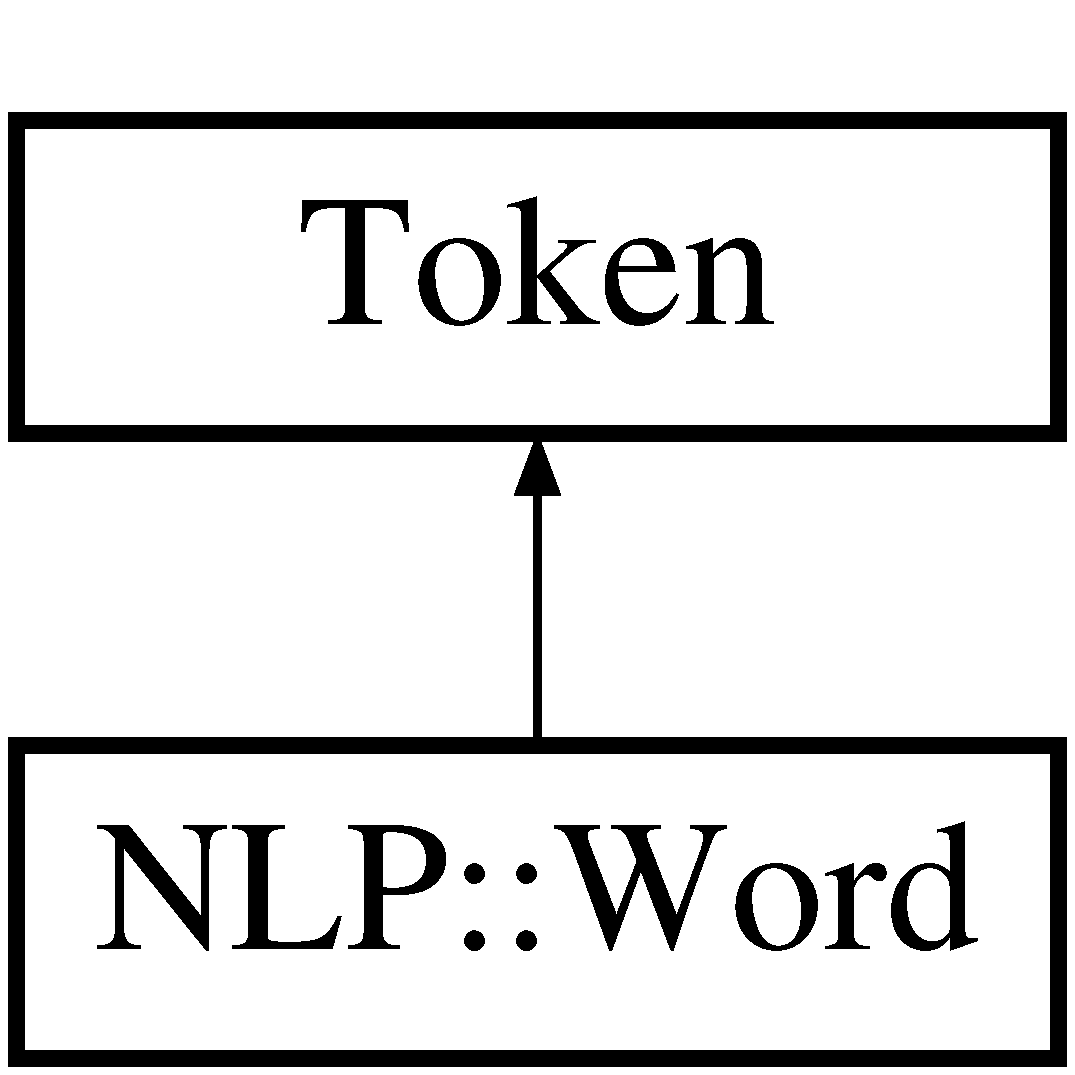
\includegraphics[height=2.000000cm]{classToken}
\end{center}
\end{figure}
\subsection*{Public Member Functions}
\begin{DoxyCompactItemize}
\item 
\hypertarget{classToken_a28857fe5c15e75db89ef881dd5a90bea}{{\bfseries Token} (const \hyperlink{classToken}{Token} \&other)}\label{classToken_a28857fe5c15e75db89ef881dd5a90bea}

\item 
\hyperlink{classToken_aeadc72fcf9d09263a0b389a0be75da01}{Token} (string s, Token\-Type type)
\begin{DoxyCompactList}\small\item\em Constructor for \hyperlink{classToken}{Token}. \end{DoxyCompactList}\item 
\hypertarget{classToken_ab21a83f4980dda611ef90d256ad97247}{{\bfseries Token} (char ch, Token\-Type type)}\label{classToken_ab21a83f4980dda611ef90d256ad97247}

\item 
\hypertarget{classToken_ae5f14af971e4c134f8ee4bec6e4a7a90}{Token\-Type {\bfseries get\-Type} () const }\label{classToken_ae5f14af971e4c134f8ee4bec6e4a7a90}

\item 
\hypertarget{classToken_a747191a1624f99f687e1827d42f81c2a}{string {\bfseries get\-Token\-String} () const }\label{classToken_a747191a1624f99f687e1827d42f81c2a}

\item 
\hypertarget{classToken_a6d59126590e655d6927239d127bcd083}{\hyperlink{classToken}{Token} \& {\bfseries operator=} (const \hyperlink{classToken}{Token} \&new\-Token)}\label{classToken_a6d59126590e655d6927239d127bcd083}

\item 
\hypertarget{classToken_a4d1f55521bbe30c59828530a3c3b3923}{const string \& {\bfseries operator$\ast$} ()}\label{classToken_a4d1f55521bbe30c59828530a3c3b3923}

\end{DoxyCompactItemize}
\subsection*{Protected Attributes}
\begin{DoxyCompactItemize}
\item 
\hypertarget{classToken_a8573f395d35b576052792fb9bad960ff}{string {\bfseries m\-Token\-String}}\label{classToken_a8573f395d35b576052792fb9bad960ff}

\item 
\hypertarget{classToken_a5d8494a08d1d8af466b7a324ae0de7b7}{Token\-Type {\bfseries m\-Type}}\label{classToken_a5d8494a08d1d8af466b7a324ae0de7b7}

\end{DoxyCompactItemize}
\subsection*{Friends}
\begin{DoxyCompactItemize}
\item 
\hypertarget{classToken_a1b93f108f6112a09c579ff23eabaacfa}{ostream \& {\bfseries operator$<$$<$} (ostream \&outs, const \hyperlink{classToken}{Token} \&t)}\label{classToken_a1b93f108f6112a09c579ff23eabaacfa}

\end{DoxyCompactItemize}


\subsection{Constructor \& Destructor Documentation}
\hypertarget{classToken_aeadc72fcf9d09263a0b389a0be75da01}{\index{Token@{Token}!Token@{Token}}
\index{Token@{Token}!Token@{Token}}
\subsubsection[{Token}]{\setlength{\rightskip}{0pt plus 5cm}Token\-::\-Token (
\begin{DoxyParamCaption}
\item[{string}]{s, }
\item[{Token\-Type}]{type}
\end{DoxyParamCaption}
)}}\label{classToken_aeadc72fcf9d09263a0b389a0be75da01}


Constructor for \hyperlink{classToken}{Token}. 


\begin{DoxyParams}{Parameters}
{\em string,type} & \\
\hline
\end{DoxyParams}
\begin{DoxyReturn}{Returns}
none 
\end{DoxyReturn}


The documentation for this class was generated from the following files\-:\begin{DoxyCompactItemize}
\item 
Tokenizer/token.\-h\item 
Tokenizer/token.\-cpp\end{DoxyCompactItemize}

\hypertarget{classNLP_1_1Word}{\section{N\-L\-P\-:\-:Word Class Reference}
\label{classNLP_1_1Word}\index{N\-L\-P\-::\-Word@{N\-L\-P\-::\-Word}}
}


A Class to store token and its corresponding tags and definitions.  




{\ttfamily \#include $<$word.\-h$>$}

Inheritance diagram for N\-L\-P\-:\-:Word\-:\begin{figure}[H]
\begin{center}
\leavevmode
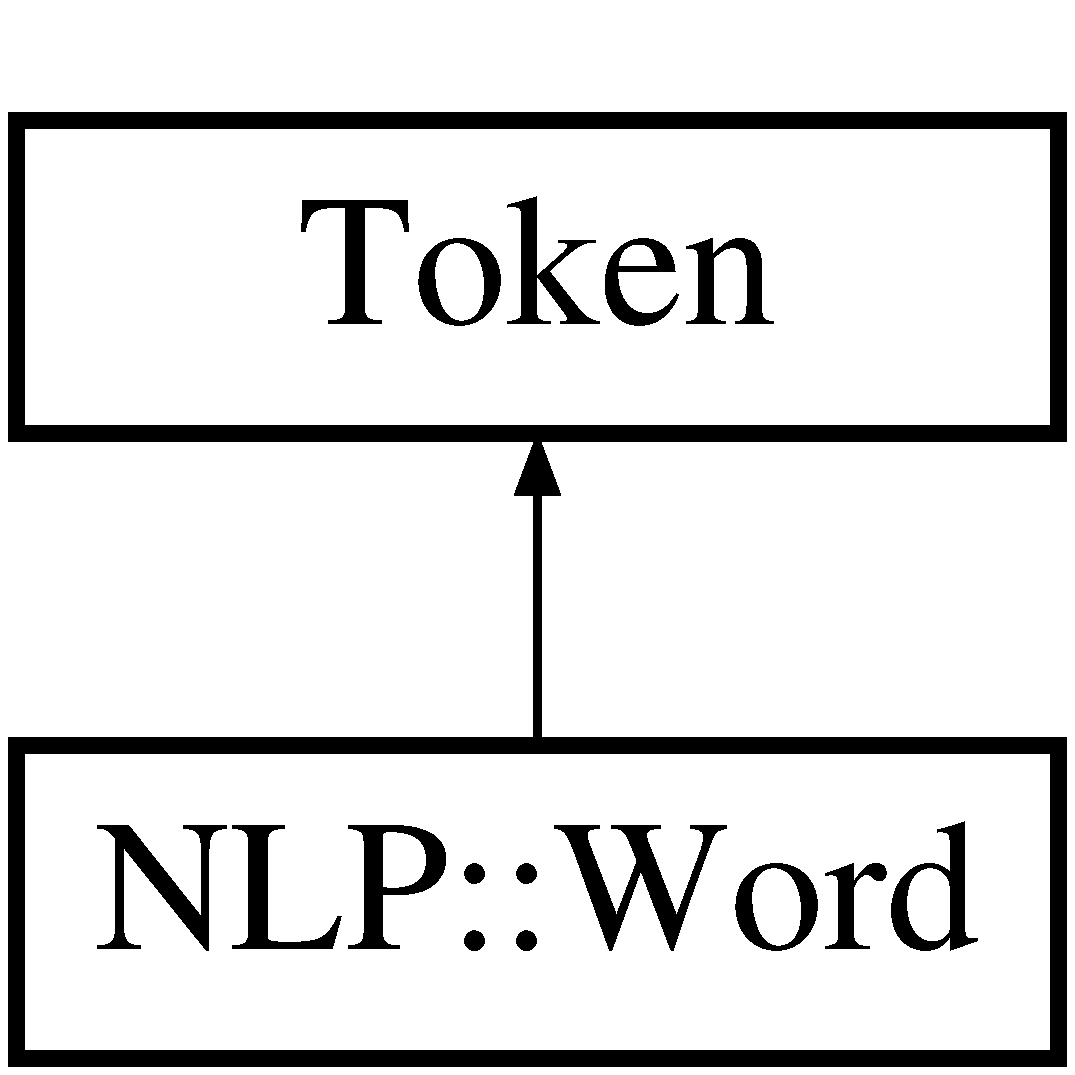
\includegraphics[height=2.000000cm]{classNLP_1_1Word}
\end{center}
\end{figure}
\subsection*{Public Member Functions}
\begin{DoxyCompactItemize}
\item 
\hypertarget{classNLP_1_1Word_ab3c1ee97a462ae81d2beb6036b0e6464}{{\bfseries Word} (const \hyperlink{classToken}{Token} \&other, set$<$ Word\-Type $>$ tags, set$<$ string $>$ defs=set$<$ string $>$())}\label{classNLP_1_1Word_ab3c1ee97a462ae81d2beb6036b0e6464}

\item 
\hypertarget{classNLP_1_1Word_a1d3d8d0a6a2483459a343c6826bd9a1d}{{\bfseries Word} (const \hyperlink{classNLP_1_1Word}{Word} \&other)}\label{classNLP_1_1Word_a1d3d8d0a6a2483459a343c6826bd9a1d}

\item 
\hypertarget{classNLP_1_1Word_a031a3d38663f2475cb1a2cdd8f913a5f}{\hyperlink{classNLP_1_1Word}{Word} \& {\bfseries operator=} (const \hyperlink{classNLP_1_1Word}{Word} \&new\-Token)}\label{classNLP_1_1Word_a031a3d38663f2475cb1a2cdd8f913a5f}

\item 
\hypertarget{classNLP_1_1Word_ae0532af7d6dd1af235d9905fb05180ef}{\hyperlink{classNLP_1_1Word_ae0532af7d6dd1af235d9905fb05180ef}{$\sim$\-Word} ()}\label{classNLP_1_1Word_ae0532af7d6dd1af235d9905fb05180ef}

\begin{DoxyCompactList}\small\item\em Do nothing. \end{DoxyCompactList}\item 
\hypertarget{classNLP_1_1Word_a8b9f67069d067c9f1f95a7db47f34fca}{string {\bfseries get\-Name} () const }\label{classNLP_1_1Word_a8b9f67069d067c9f1f95a7db47f34fca}

\item 
\hypertarget{classNLP_1_1Word_a5249b40d5a2c47b358ba62eb50fc9487}{set$<$ Word\-Type $>$ {\bfseries get\-Types} () const }\label{classNLP_1_1Word_a5249b40d5a2c47b358ba62eb50fc9487}

\item 
\hypertarget{classNLP_1_1Word_a08390797ca3573623becf73a8ac97dba}{string {\bfseries get\-Rawtypes} () const }\label{classNLP_1_1Word_a08390797ca3573623becf73a8ac97dba}

\item 
\hypertarget{classNLP_1_1Word_a2e5b2960a52245f6581183d02e823cf8}{set$<$ string $>$ {\bfseries get\-Definitions} () const }\label{classNLP_1_1Word_a2e5b2960a52245f6581183d02e823cf8}

\end{DoxyCompactItemize}
\subsection*{Friends}
\begin{DoxyCompactItemize}
\item 
\hypertarget{classNLP_1_1Word_a59a0b91ac5b87e8c5fc042105f99a1a0}{ostream \& {\bfseries operator$<$$<$} (ostream \&outs, const \hyperlink{classNLP_1_1Word}{Word} \&w)}\label{classNLP_1_1Word_a59a0b91ac5b87e8c5fc042105f99a1a0}

\end{DoxyCompactItemize}
\subsection*{Additional Inherited Members}


\subsection{Detailed Description}
A Class to store token and its corresponding tags and definitions. 


\begin{DoxyParams}{Parameters}
{\em public} & \\
\hline
\end{DoxyParams}


The documentation for this class was generated from the following files\-:\begin{DoxyCompactItemize}
\item 
Tagger/word.\-h\item 
Tagger/word.\-cpp\end{DoxyCompactItemize}

%--- End generated contents ---

% Index
\newpage
\phantomsection
\addcontentsline{toc}{chapter}{Index}
\printindex

\end{document}
